\documentclass[aspectratio=43]{beamer}
\usepackage[utf8]{inputenc}

%%%%%%%%%%%%%%%%%%%%%%%% THEME
\usetheme{material}
\useLightTheme
\usePrimaryAmber
\useAccentDeepOrange

\usepackage{macros} % must come after theme

\title{\q Search}
\keywords{\qc, \q Search, Grover's algorithm}

\begin{document}

\begin{frame}
	\titlepage
\end{frame}


\begin{frame}{Table of contents}
	\begin{card}
		\tableofcontents
	\end{card}
\end{frame}


\section{Introduction}
\begin{frame}{Introduction}
    \begin{card}
        This week we will be studying a famous and pragmatic quantum algorithm to perform a search, the \textbf{\gvsa}. We will look through its purpose, how it compares with classical search strategies that solve the same problems. The algorithm will be studied from a more abstract point of view, namely in understanding \textbf{\aamp} (\textbf{\phiv} + \textbf{\iatm}). This week's exercises will focus more on the implementation details.
    \end{card}
\pagenumber
\end{frame}


\section{The Search Problem}
\begin{frame}{The Search Problem}
    \begin{cardTiny}
        Let us assume we have a function $f$:
        \begin{equation*}
            f : \{0, 1, ..., N-1\} \rightarrow \{0,1\}
        \end{equation*}
        And we want to find those values of $x$ for which $f(x)=1$. To simplify, and also to make the problem harder, let us assume there is only one such $x$:
    \begin{center}
        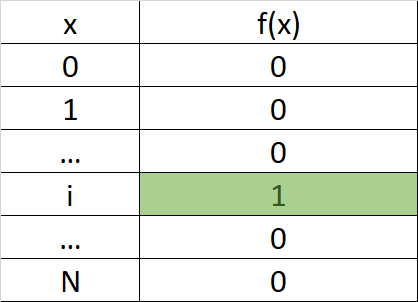
\includegraphics[width=0.45\textwidth]{haystack}
    \end{center}
    \end{cardTiny}
\pagenumber
\end{frame}

\begin{frame}{The Search Problem}
    \begin{card}
        How would a classical programmer tackle this problem?
        \begin{itemize}
            \item Sequential search through $x \in [0, N[$ until $f(x)=1$
            \item Random search with $x \in [0, N[$ until $f(x)=1$
            \item ...
        \end{itemize}
        As you can see, this is quite straightforward, and yields a worst-case scenario of $N$ searches and average $\frac{N}{2}$ (assuming no bias in $f$).
    \end{card}
\pagenumber
\end{frame}

\section{SAT Problem}
\begin{frame}{SAT Problem}
    \begin{card}
        \small{Besides the most obvious problems, we should also know about the \textbf{SAT problem} (sometimes Boolean satisfiability problem). This problem is about determining values for Boolean variables so that the \textbf{Boolean expression} associated \textbf{evaluates to true}. This is a computationally expensive problem and falls into the \np (actually \href{https://en.wikipedia.org/wiki/NP-completeness}{NP-complete}) category. Many problems, like scheduling, can be converted into a SAT formulation, making use of existing SAT solvers to easily find solutions for novel problems.}
    \end{card}
    \begin{card}
        \small{As such, SAT can be seen as a \textbf{search problem}, where we need to find the precise combination of Boolean values that \textbf{yields true}.}
    \end{card}
\pagenumber
\end{frame}

\section{\gvsa} % overview of steps, comparison of bigO
\begin{frame}{\gvsa}
    \begin{card}
        Luckily for the world, Dr. \href{https://en.wikipedia.org/wiki/Lov_Grover}{Lov Grover} devised an algorithm that, instead of $N$ steps to find a solution, requires $\sqrt{N}$. This is a \href{https://arxiv.org/abs/quant-ph/9711070}{it is optimal} (no better speed up is possible for this problem). 
    \end{card}
    \begin{card}
        The algorithm makes use of two very important phenomenon that can be implemented in a quantum computer:\begin{itemize}
            \item \textbf{Phase inversion}
            \item \textbf{Inversion about the mean} (average)
            \item An oracle for our $f$ function
        \end{itemize}
    \end{card}
\pagenumber
\end{frame}


\section{Phase Inversion}
\begin{frame}{Phase Inversion}
    \begin{card}
        The first phenomena is that of \phiv and will help in finding $x'$ so that $f(x')=1$. Let us imagine a quantum superposition over all possible $x$ values:
        \begin{equation*}
            \sum_x\alpha_x \ket{x}
        \end{equation*}
        To which we can, through the use of our oracle, obtain:
        \begin{equation*}
            \sum_{x\neq x'}\alpha_x \ket{x} - \alpha_{x'}\ket{x'}
        \end{equation*}
    \end{card}
\pagenumber
\end{frame}
\begin{frame}{Phase Inversion}
    \begin{cardTiny}
        This will mean that, if we plot $\alpha_x$ for each $x$ value, we will get something like the following abstract diagram - in which the real value has been inverted (even though we do not know its value)
        \begin{multicols}{2}
            \begin{center}
                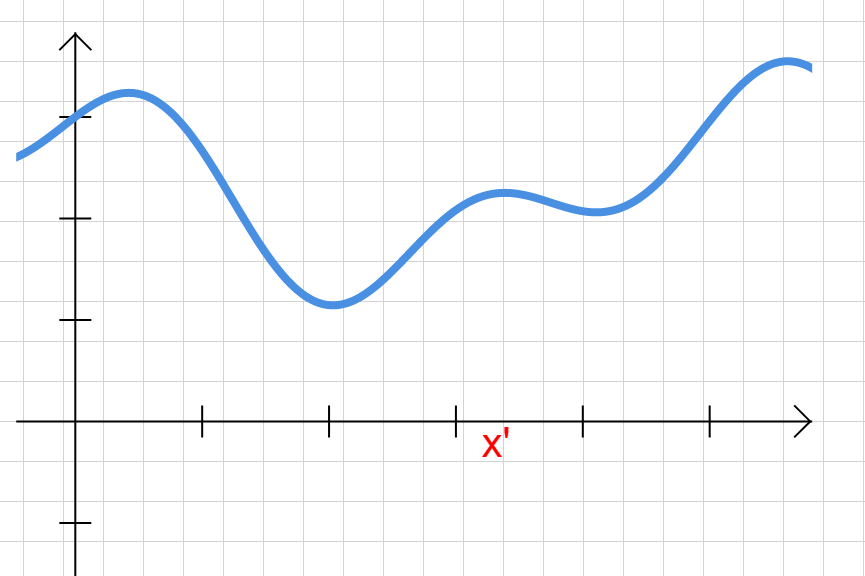
\includegraphics[width=0.5\textwidth]{phiv_before}
            \end{center}
            \begin{center}
                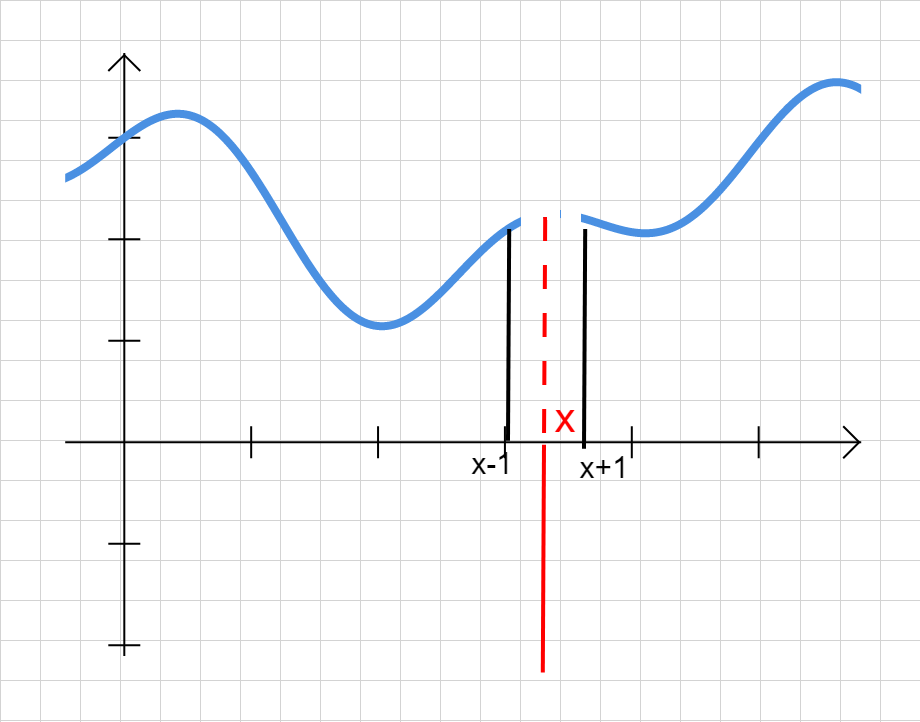
\includegraphics[width=0.5\textwidth]{phiv}
            \end{center}
        \end{multicols}
    \end{cardTiny}
\pagenumber
\end{frame}


\section{Inversion about the Mean}
\begin{frame}{Inversion about the Mean}
    \begin{cardTiny}
    The next phase of the algorithm is to take that very distribution of weight and mirror it to the other side of the mean. This can be done in a quantum circuit (more on the exercises). The following is a representation of this transformation (either function is the \iatm of the other):
    \begin{center}
        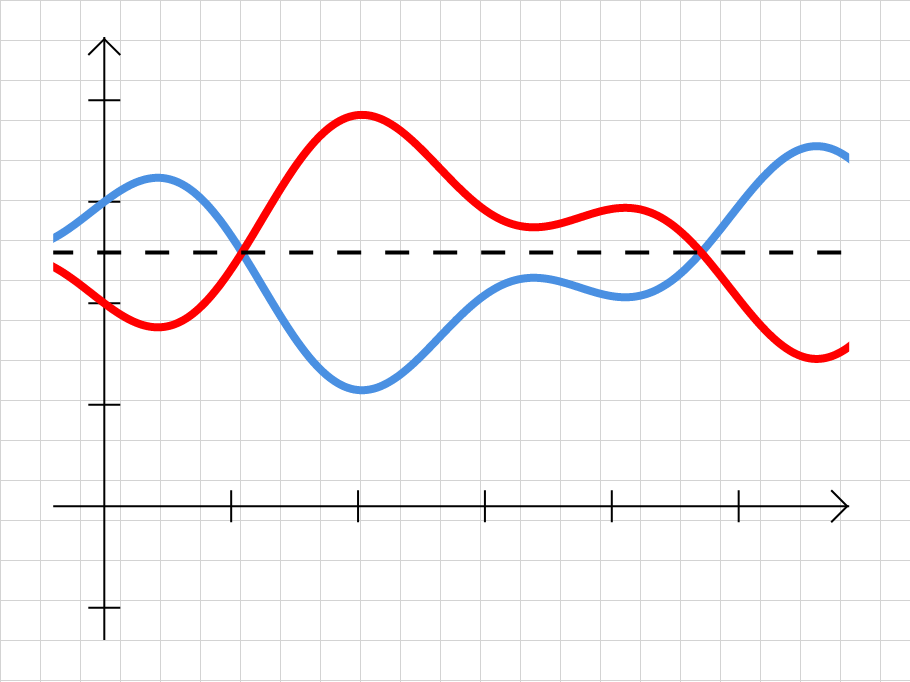
\includegraphics[width=0.5\textwidth]{iatm}
    \end{center}
    \end{cardTiny}
\pagenumber
\end{frame}

\begin{frame}{Inversion about the Mean}
    \begin{cardTiny}
        Why do we do this, you may ask. To answer this, consider the two steps taken so far: \phiv and then \iatm. The first one, sets our solution to be a bit more recognizable and the second operation further segregates our result from the rest of the possible states.
    \end{cardTiny}
    \begin{cardTiny}
        If we keep on doing this two steps, we will segregate the correct answer from the others further and further. The number of times we need to do it to have a guaranteed high probability of having the right answer is $\sqrt{N}$!
    \end{cardTiny}
\pagenumber
\end{frame}

\section{Why $\sqrt{N}$?}
\begin{frame}{\gvsa (why $\sqrt{N}$?) }
    \begin{cardTiny}
        Let us assume, we initialize our $n$ qubits to $\ket{0}$, each qubit can be compared to a Boolean value on the n-bit solution we are looking for. We then create a superposition that sets them in a \textbf{uniform superposition} (each state has equal probability):
        \begin{equation*}
            \sum_{x \in {0,1}^n} \frac{1}{\sqrt{N}}\ket{x}
        \end{equation*}
        \begin{center}
            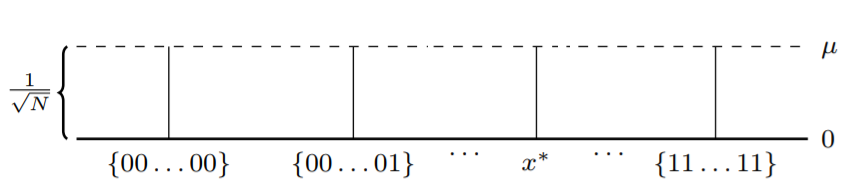
\includegraphics[width=1\textwidth]{grover_start}
        \end{center}
    \end{cardTiny}
\pagenumber
\end{frame}


\begin{frame}{\gvsa (why $\sqrt{N}$?)}
    \begin{cardTiny}
        We then create a quantum oracle $O_f$ that will flip the qubits if the result is 1, and apply this gate, this effectively applies a phase inversion:
        \begin{center}
            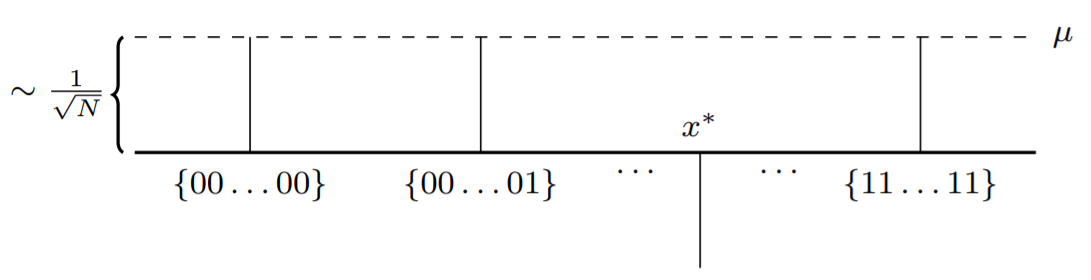
\includegraphics[width=1\textwidth]{grover_phiv}
        \end{center}
    \end{cardTiny}
\pagenumber
\end{frame}

\begin{frame}{\gvsa (why $\sqrt{N}$?)}
    \begin{cardTiny}
        Finally, we will apply the \iatm ($\mu = \frac{1}{N}\sum_x \alpha_x \ket{x}$):
        \begin{equation*}
            \sum_x \alpha_x \ket{x} \rightarrow \sum_x (2\mu - \alpha_x) \ket{x}
        \end{equation*}
        \begin{center}
            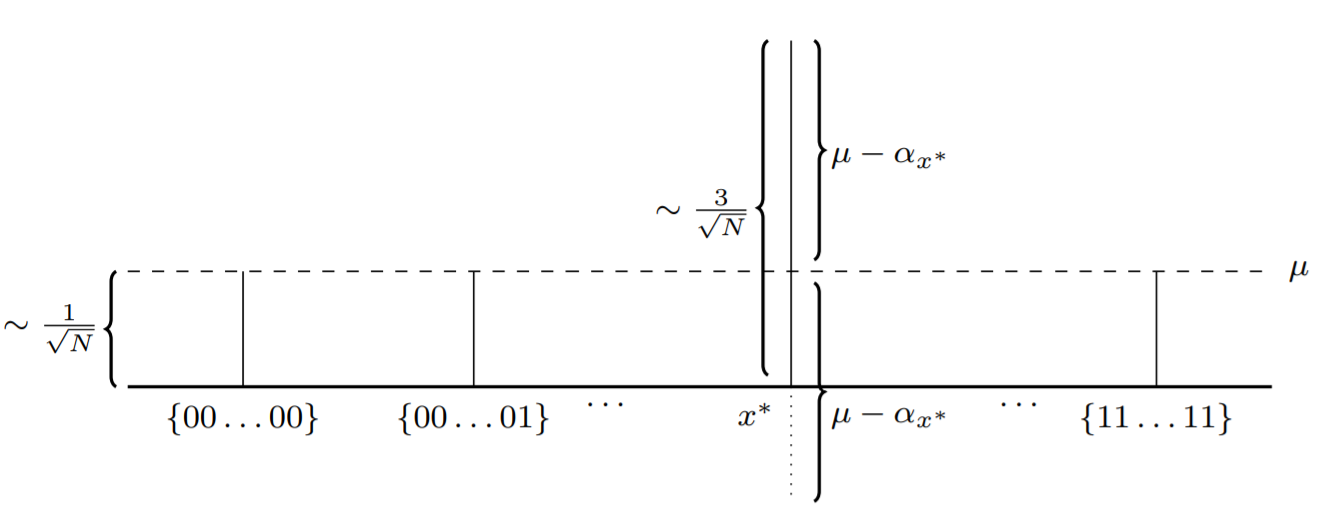
\includegraphics[width=1\textwidth]{grover_iotm}
        \end{center}
    \end{cardTiny}
\pagenumber
\end{frame}

\newcommand{\amp}[2]{\frac{#1}{\sqrt{#2}}}
\begin{frame}{\gvsa ($\sqrt{N}$ because...)}
    \begin{card}
        If you repeat this mechanism, you will notice the amplitude improves (per step) $\amp{\sqrt{2}}{N}$ every iteration:
        \begin{equation*}
            \amp{1}{N}, \amp{3}{N}, \amp{5}{N}, ... \amp{1}{2}
        \end{equation*}
        At the point of $\amp{1}{2}$ we have a guaranteed high probability of the measurement resulting in the solution! How long until we get there?
        \begin{equation*}
            \frac{\amp{1}{2}}{\amp{\sqrt{2}}{N}} = \frac{\sqrt{N}}{2} = O(\sqrt{N})
        \end{equation*}
    \end{card}
\pagenumber
\end{frame}

\section{\aamp}
\begin{frame}{\aamp}
    \begin{cardTiny}
        This combination of \phiv and \iatm is called \textbf{\aamp}!
    \end{cardTiny}
    \begin{cardTiny}
        \small{
        It should be noted that the amplitude \textbf{cannot increase forever} and will eventually be so large that the mean becomes negative (after \phiv) and the \iatm step is actually \textbf{harming our result}. That is why one should know hen to stop (how many iterations guarantee the minimum desired amplitude).}
    \end{cardTiny}
    \begin{cardTiny}
        There you have it, by executing the \aamp iteration we can solve a classical problem that had a complexity of $O(N)$ in $O(\sqrt{N})$, it is not an exponential growth (as some quantum algorithms are able to do), but in this case that would have some \href{https://en.wikipedia.org/wiki/P_versus_NP_problem}{very disruptive consequences}. 
    \end{cardTiny}
\pagenumber
\end{frame}

\section{Hands-on}
\begin{frame}{Hands-on}
    \begin{card}
        This week's exercises will focus more on understanding the logic at the quantum circuit level, and are based on a Jupyter notebook available at the official \href{https://github.com/Qiskit/qiskit-tutorial}{\qk tutorial repository}. You will get to solve a real SAT problem, of dimension 3, in a real quantum device!
    \end{card}
\pagenumber
\end{frame}

\section{Where to learn more?}
\begin{frame}{Where to learn more?}
\begin{card}
    \begin{itemize}
        \item \href{https://quantumexperience.ng.bluemix.net/proxy/tutorial/full-user-guide/004-Quantum_Algorithms/070-Grover's_Algorithm.html}{\ibmqe Documentation on \gv} includes circuitry and interesting diagrams.
        \item \href{https://arxiv.org/abs/1708.03684}{An Introduction to Quantum Computing, Without the Physics} good paper for understanding more on \gvsa
    \end{itemize}
\end{card}
\end{frame}
\end{document}
